\chapter{Efficient Factor Graph Fusion}
\label{chap:three}

%In order to be useful for the mobile robots, SLAM needs to perform at real-time. Solving the SLAM problem represented by a factor graph proceeds by optimizing the equivalent nonlinear least-squares problem \cite{lumiliosfirstgraphslam}. The sparsity of the underlying graph structure makes the optimization tractable at real-time. During factorization the sparsity of the graph is retained using a technique widely known in the sparse linear algebra and graph theory community called variable reordering. Variable ordering or Elimination ordering is the order in which the variables are eliminated while solving a system of linear equations. A good ordering is necessary to avoid fill-in which refers to the additional non zero entries produced out of factorization. In case of a multi-robot scenario, factor graphs of the individual robots are fused/combined to improve the overall estimate. This requires finding the variable ordering of the fused factor graph. 
%Chapter 3 comes up with a methodology to quickly find the variable ordering of the combined graph using the ordering of the participating factor graphs. The worst case here would be to do a complete reordering of the fused graph. We provide a complexity analysis to compare the time performance of both the options. Also, fusing and factorizing the graph during multi-robot SLAM optimization for best estimate requires coming up with a variable ordering for the fused graph. Factorizing/Solving a factor graph proceeds by generating a order of elimination for the variables called variable ordering or elimination ordering. In case of a multi-robot scenario while combining the factor graphs to improve the overall estimate the variable ordering of the participating factor graphs can be used to quickly find the variable ordering of the resultant combined factor graph. To do this, we use the Bayes Tree \cite{kaessbayestree} representation of the factor graph which also gives access to the subset of variable that gets affected on combining the parent factor graphs. 
In the previous chapter, I described how the multi-robot smoothing and mapping is formulated as a least squares problem with a flavor that is specific to our implementation. Following that, I discussed the options to incrementally solve the least squares optimization and the critical requirement for fast, efficient and incremental variable reordering. A good ordering is necessary to reduce the amount of fill-in which refers additional non-zeros introduced during elimination. However, it has been shown that finding an optimal ordering for an arbitrary factor graph is NP-complete \cite{orderingnphard}. An optimal ordering called perfect elimination ordering \cite{chordaloptimalordering} exists only if the factor graph is chordal. SLAM graphs are generally \textit{not} chordal mainly due to revisiting the landmarks after a long time and loop closures that connect two far away nodes. Loops in the trajectory can result in a significant increase in computational complexity through a large increase of non-zero entries in the factor matrix. In addition to the typical loop closures in the SLAM problem, a multi-robot scenario could introduce several non-trivial loop closures. This is because for an indirect encounter between the robots, a big chunk of graph with several measurements from one robot has to combined with a far away node of another robot. Such an update is equivalent to loop closure in terms of computation and storage. Despite that, it is important in a multi-robot scenario to fuse the factor graphs of individual robots to improve the overall estimate. This requires finding the variable ordering of the fused factor graph.
\paragraph{}
To combat this scenario, this chapter comes up with a methodology to quickly find the variable ordering of the combined graph using the ordering of the participating factor graphs. The worst case here would be to do a complete reordering of the fused graph. We provide a complexity analysis to compare the time performance of both the options. The outline of this chapter is as follows: In the next section, I will provide a relevant literature survey from linear algebra and graph theory community. Following that, I will dive deep in to Bayes tree data structure that was introduced in the previous chapter to establish incremental variable ordering. Then I will formally verify that the proposed ordering does not violate any of the standard rules to be obeyed. Finally, I will explain the proposed approach and display results on a standard dataset from sparse linear algebra community.

\section{Related Work} 
Solving the least-squares and linear programming problem is central to several scientific  and engineering applications. Our focus in on sparse least-squares optimization with primary applications to SLAM. Smoothing formulation of SLAM as a least-squares with sparse graphs was first done by Lu and Milios \cite{lumiliosfirstgraphslam}. Their method provides both batch and sequential procedure but performs the expensive inversion of the information matrix for updates. Although several smoothing based SLAM solutions have been developed based on conjugate gradient \cite{cgdescent}, gradient descent \cite{gdescent}, relaxation \cite{thrunprobabilistic} and multi-level relaxation \cite{mlrelaxation}, we only deal with the ones that derive performance improvements from information matrix decomposition. $\sqrt{SAM}$ by Dellaert \cite{dellaertonlysam} was the first work to replace expensive matrix inversion with sparse matrix factorization for the SLAM problem. It mentioned the dramatic performance improvements that could be derived from good variable ordering but is done only on a batch setting. The two key algorithms that improved on the least-squares formulation of SLAM using the premise set by \cite{dellaertonlysam} include ISAM \cite{kaessisam} and ISAM2 \cite{kaessisam2}. Both of these works combine the formulation in \cite{lumiliosfirstgraphslam} with the interchangeable linear algebra and graph theory flavor introduced in \cite{dellaertonlysam} and provide some additional improvements in terms of incremental optimization. Recently, Agarwal and Olson \cite{variableorderingslam} provided different variable reordering strategies to SLAM and explained the critical role played by variable ordering in different solutions to SLAM. 
\paragraph{}
In our work, we use ISAM2 using the Bayes tree \cite{kaessbayestree} \cite{kaessisam2} as the underlying state estimation engine because it is exact, incremental and solves the full non-linear problem. While tremendous amount of work is done to extend the general SLAM algorithms to multiple robots, smoothing and mapping for multi-robot SLAM is not explored much. The most relevant ones include \cite{multipleisam} by Kim \textit{et al.}, C-SAM \cite{csam} and Tectonic SAM \cite{tectonicsam}. Although these algorithms are based on Smoothing and Mapping, Tectonic SAM addresses only single robot, batch mapping and the other two algorithms only address the fundamental multi-robot mapping issues like map-aligning and relative pose initialization. Important graph based SLAM approaches that build independent sub-graphs and merge those graphs include \cite{gdescent}, \cite{fresetreemap} and \cite{freseclosing}.  Folkesson's \cite{gdescent} reduces the graph complexity by collapsing parts of the robot trajectory into a cluster called star-nodes. Frese's \cite{fresetreemap} and \cite{freseclosing} gives a hierarchical approach by exploiting the square root information and representing the Cholesky factors as a tree data structure. They provide a highly efficient algorithm but employ numerous approximations and none of these partition based algorithms are extended to multi-robots. Also, several recent developments in the algebraic graph theory community like hypergraph nested dissection ordering \cite{hund} and exact graph partitioning algorithm \cite{exactordering} have not been utilized in solutions for SLAM. Clearly from the above discussion, previous research has either been done in graph merging for single robot SLAM or, multi-robot SLAM that does not deal with combining the graphs. 
\paragraph{}
While solving large linear systems, it is a very common preprocessing step to order the columns of the matrix $A$ to be factorized to keep the factorization as sparse as possible. Finding the variable ordering involves finding the permutation matrix $P$ which is right-multiplied with $A$ to obtain the ordered matrix $AP$. Cholesky or QR factorization of $AP$ is more sparser and requires less storage than factorizing $A$. Ordering schemes have been proposed for different class of problems that include - 1) $A$ being symmetric 2) $A$ being unsymmetric. As finding the optimal ordering is NP-complete \cite{orderingnphard} various heuristics have been developed. The common aspect across all the approaches is to eliminate the nodes in the ascending order of their degrees. This is called as the minimum degree algorithm which is derived from a method first proposed by Markowitz in 1957 \cite{markowitzelimination} for non-symmetric linear programming problems. The symmetric matrix version was formalized by Tinney \textit{et al.} \cite{tinneyfirstordering}. The ordering of the nodes directly on the graph data structure was derived by Rose \cite{rosegraph}. Initial algorithms for symmetric matrices also include approximate minimum degree (AMD) \cite{amd} and nested dissection \cite{nesdis}. In case of the unsymmetric matrix such as Jacobian $A$, it is converted to symmetric information form $A^\top A$ to be used by these ordering schemes. State-of-the-art algorithms like column approximate minimum degree ordering (COLAMD) \cite{colamd} works directly on the non-zero pattern of $A$ without explicitly calculating $A^\top A$. A brief survey of the evolution of minimum degree ordering is consolidated by George \cite{georgeevolution}. Nested dissection is a divide and conquer heuristic based on graph partitioning that has the advantage of reordering the matrix into a form suitable for parallel execution. Very recently, nested dissection has been extended to unsymmetric hypergraphs in \cite{hund}. Although there is a significant amount of research in developing a near to optimal variable ordering tailored for various graphical models, to the best of our knowledge, there is no work in finding an ordering for the graph obtained by fusing ordered graphs. 

\section{Bayes Tree for Variable Ordering}
Topologically, the Bayes net described in Section \ref{sss:bayes_net_intro} is a chordal directed acyclic graph. By identifying cliques (groups of fully connected variables), the Bayes net may be rewritten as a Bayes tree. For full details about the clique-finding algorithm, see Kaess et al. \cite{kaessbayestree}. Within the Bayes tree, each node represents the conditional density of the clique variables (also called as frontal variables), $\Theta_j$, given all of its neighbors (also called as separators), $N(\Theta_j)$:
\begin{equation}
p(\Theta) = \Pi(\Theta \mid N(\Theta_j))
\end{equation}
During elimination of the factor graph (assuming the Bayes net is formed), the leaves of the tree are built first, and factors on the conditional variables are passed up the tree to their parents. Back-substitution then proceeds top-down from the root clique, which is eliminated last, as it has no external dependencies. The solution of the frontal variables of the parent clique are passed down the tree to the children, which are guaranteed to depend only on the frontal variables of their ancestors. 
\begin{figure}
\centering
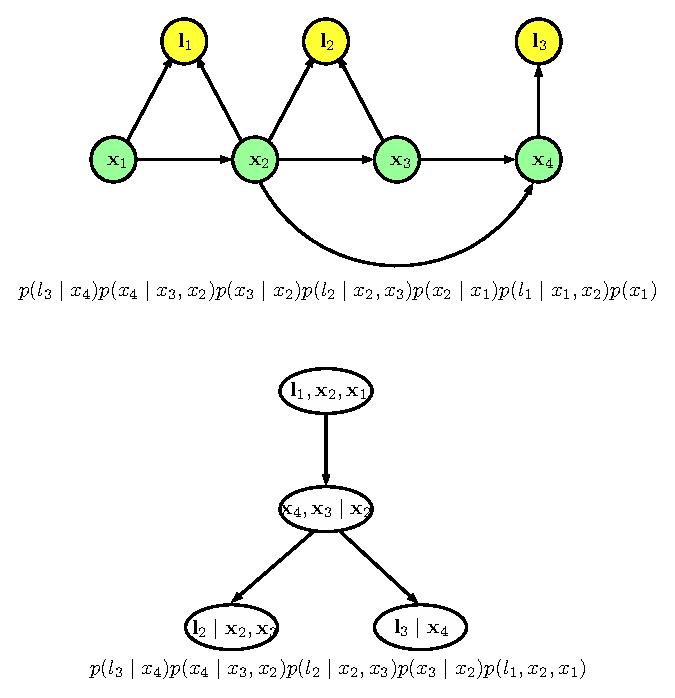
\includegraphics{Chapters/figures3/bn_bt_factorization_vert}
\caption{Bayes network and Bayes tree representations of the factor graph example used in last chapter with the elimination order $O = [l_3, l_2, l_1, x_4, x_3, x_2, x_1]$. The factorization of the factor graph joint probability density is mentioned for both the representations.}
\label{fig:bn_bt_factorization}
\end{figure}
\paragraph{}
Like the Bayes net, the structure of the Bayes tree is affected by the selected variable ordering. The Bayes net and Bayes tree representations are interchangeable. This is shown in the Figure \ref{fig:bn_bt_factorization} with the factor graph example used in Section \ref{ss:fg_to_bn_to_bt}. The terms $p(l_3\mid x_4)$, $p(x_4 \mid x_3, x_2)$, $p(x_3 \mid x_2)$, $p(l_2 \mid x_2, x_3)$ are present in both the factorizations. It can be shown using the chain rule in Bayes theorem that $p(l_1, x_2, x_1) = p(l_1 \mid x_1,x_2)p(x_2\mid x_1)p(x_1)$. Although both the representations are same given the variable ordering, modeling the inference using a tree structure is often more convenient and intuitive: elimination passes information up the tree, while back-substitution propagates information down the tree.
\paragraph{}
At every iteration, the update can be a new variable to be added to the graph or a new measurement factor connecting already existing variables. In both the cases, the square-root information of several variables other than the new variable in different cliques of the Bayes tree has to be updated. This could either be done by 1) Going back to the factor graph, adding a new measurement and/or a variable, reordering all the variables and completely factorizing the graph from scratch or 2) Partially recovering the portion of factor graph to which the new measurement and/or a variable should be added, reordering the partial graph and factorizing it. The second option is incremental, efficient and hence preferable, but would require the knowledge of subset of variables and factors that gets affected on touching a variable. This is exactly obtainable from the formulation of the Bayes tree.
\paragraph{}
A new variable is always accompanied by a measurement. When a new measurement is added, for example a factor $c^\prime(x_j,x_{j^\prime})$, only the paths between the cliques containing $x_j$ and $x_{j^\prime}$ (respectively) and the root are affected. The sub-trees below these cliques are unaffected, as are any other sub-trees not containing $x_j$ or $x_{j^\prime}$. The example in Figure \ref{fig:bt_add_var} demonstrates the addition of a new pose node to the factor graph and Bayes tree example used in the previous chapter in Figure \ref{fig:bn_to_bt}.
\begin{figure}
\centering
\includegraphics[width=\textwidth]{Chapters/figures3/bt_add_new_variable}
\caption{Adding a new variable with measurement to a factor graph example described in the previous chapter. It should be noted that only a part of the Bayes tree (red filled nodes) to which the new variable is added is recovered, reordered and factorized. The unaffected cliques (purple filled nodes) are attached back to the new tree. The new variable added is shown used a red broken circle.}
\label{fig:bt_add_var}
\end{figure}
\paragraph{}
This in turn may move the estimates far off the current linearization point or add new non-zero components to the square-root factor. The former would require updating the linearization point and the latter requires reordering the variables. But as the set of variables that will be affected is known in advance it could be leveraged by changing the linearization point or reordering and factorizing only those variables. This relationship is understood by the construction of Bayes tree and was not obvious within the matrix framework \cite{kaessbayestree}.  
\subsection{Multi-robot Pose Graph Fusion}
From the construction of the Bayes tree discussed so far and the example in Figure \ref{fig:bt_add_var} it is clear that the Bayes tree is suitable for updating the square-root information incrementally. With ISAM2 \cite{kaessisam2} as the SLAM algorithm, a centralized cooperative mapping system will require fusing the maps from individual robots represented as the Bayes tree. In case of centralized mapping it could be assumed that every robot's factor graph is accessible always with no restrictions on bandwidth or that the robots share information only when they encounter. For our experiment, we assume that the robots share information only when they encounter. Also, our procedure does not require both the robots to identify each other when they encounter and work even if one robot identifies the other. Knowing the subset of variables using the Bayes tree which alone can be reordered could easily be extended to the situation of fusing multiple robots' pose graphs. 
\paragraph{}
Direct encounters between robots introduce a constraint between the cliques of two different Bayes tree with pose nodes as the frontal variables. As a direct encounter relates the recent pose of the robots, the constraint joins the nodes near the root of the tree. The argument that the recent poses of the robot need not necessarily end up near the root of the tree after variable ordering will be addressed later. Since a connection is made between the nodes near the root of the tree the total number of affected variables is minimal. Whereas an indirect encounter occurs when two robots observe the same part of an environment (not necessarily at the same time), allowing a constraint of type robot-landmark-robot between the robot poses pivoted by the landmark pose, to be estimated. They could also be transformed into a constraint between the positions of two robots at the respective time steps. This type of constraint connects the recent pose of one of the robots from which the landmark is observed with a older pose of another robot from which the same landmark was observed. Figure \ref{fig:fusing_bt} gives a pictorial step-by-step procedure to combine two Bayes trees.
\begin{figure}
\centering
\includegraphics[height=\textheight,width=\textwidth]{Chapters/figures3/fusing_bt}
\caption{Fusing multiple Bayes trees to calculate the best estimate. Only the affected part (inside blob in row 3) of both the Bayes trees are recovered and refactorized. $O_1$, $O_2$ and $O_{fused}$ are the variable ordering of first, second and the fused factor graph.}
\label{fig:fusing_bt}
\end{figure}
\paragraph{}
In Figure \ref{fig:fusing_bt}, the factor graph of two robots exploring the environment is considered. Row 3 indicates the equivalent Bayes tree based on some variable ordering $O_1$ and $O_2$. It can be seen from the common variable among the factor graphs that both the robots have visited the same landmark $l_1$. To fuse those Bayes trees, only the path between the clique containing the landmark frontal variable and root clique is recovered as factor graph. The factor graph centred over the common variable is fused, reordered and eliminated back into a Bayes tree. The unaffected portions of the individual Bayes tree is merged back. These unaffected portions are shown as colored cliques in row 3 of Figure \ref{fig:fusing_bt}. While merging back the unaffected portions, the clique containing the earliest eliminated variable out of all the conditional variables of the unaffected clique is considered as the parent clique. For example, in Figure \ref{fig:fusing_bt}, it can be seen in the second Bayes tree that the unaffected green colored clique with frontal variable $\textbf{x}_1^2$ has two conditional variables $\textbf{x}_2^2$ and $\textbf{x}_4^2$. It is attached to the clique containing the earliest eliminated variable, according to $O_2$, as the frontal variable, $\textbf{x}_2^2$. However, in row 5 containing the fused Bayes tree, the same unaffected clique is attached to the clique with frontal variable $\textbf{x}_4^2$ as it is eliminated before $\textbf{x}_2^2$ according to $O_{fused}$. The idea here is that, during elimination information is propagated up the tree and every eliminated variable will have the variables yet to be eliminated as its ancestor if there is a fill-in between them.

\section{Formal Verification}
Before proceeding to the proposed algorithm, it is important to formally validate that the operations carried out and the utilization of Bayes tree does not violate any of the standard assumptions, works for any general class of factor graph problems and is backward compatible. Firstly, when multiple robots visit several same regions of the environment the number of common landmarks between the graphs go up. The Bayes tree would be used to extract the affected subset of variables when combining the graphs with multiple common variables. It has to be verified that these affected subset of variables do not form disconnected components. Secondly, it has to be ensured that the root clique always contains more than one frontal variable. This is needed both in terms of the property of the Bayes tree and the requirements of the software optimizer used by us, \cite{gtsamhandson}. To ensure these the following two proofs are given:
In the following write-up a variable in/of the clique usually refers to the frontal variable of the clique. Let us consider the simple case of merging two bipartite graphs $\mathcal{G}_1 = (\mathcal{C}_1, \Theta_1, \mathcal{E}_1)$ and $\mathcal{G}_2 = (\mathcal{C}_2, \Theta_2, \mathcal{E}_2)$ with their Bayes tree function given as $\mathcal{B}_i(\mathcal{C}_{i})$. The Bayes tree function returns the union of set of variables in the ancestor cliques of the clique containing each and every variable in $\mathcal{C}_{i}$, $i = 1,2$ here. The graph is merged only when the set of common variables $\mathcal{C}_1 \cap \mathcal{C}_2 \neq \emptyset$. The set of all affected variables obtained from the Bayes tree is given as $\mathcal{C}^{fused} = \mathcal{B}_1(\mathcal{C}_{1}) \cup \mathcal{B}_2(\mathcal{C}_{2}) \cup (\mathcal{C}_1 \cap \mathcal{C}_2)$. The fused graph is then given as $\mathcal{G}^{fused} = (\mathcal{C}^{fused}, \Theta^{fused} ,\mathcal{E}^{fused})$ where $\mathcal{E}^{fused} = \{ (u,w) \mid [u,w \in \mathcal{C}_1 \cap (u,w) \in \mathcal{E}_1] \cup [u,w \in \mathcal{C}_2 \cap (u,w) \in \mathcal{E}_2] \}$ and $\Theta^{fused} = \{ \theta(u,w) \mid \theta \in \Theta_1 \cup \Theta_2; u, w \in \mathcal{C}_1 \cup \mathcal{C}_2 \}$.
\begin{theorem}
The set of affected variables from the Bayes tree do not form a disconnected graph.
\end{theorem}
%\paragraph{Proof 1:} \textit{The set of affected variables from the Bayes tree do not form a disconnected graph.}\\
\begin{proof}
The common variables forming the separator when combining the factor graphs can have multiple connected components. However, the  subset of affected variables obtained by recursively traversing up the Bayes tree from every common variable forms a single connected component. It follows from the fact that, although the common variables might be present at different leaf cliques or non-leaf cliques, different branches or different depths, they all have a single root clique. Recovering all the common variables with all its ancestors will eventually be connected by the frontal variables of the root clique. It is mathematically verified by showing that the multiplicity of 0 as an eigenvalue of the Laplacian matrix of the fused graph is 1. The Laplacian matrix $\mathcal{L}_{{N\times N}}$ of a bipartite factor graph with $N$ variable nodes is given as:
\begin{equation}
\mathcal{L}^{fused} = \mathcal{D}^{fused} - \mathcal{A}^{fused}
\end{equation}
where $\mathcal{D}$ is the degree matrix and $\mathcal{A}$ is the adjacency matrix of the graph. Simplifying the above equation:
\begin{equation}
{\displaystyle \mathcal{L}_{j,k}:={\begin{cases}\deg(v_{j})&{\mbox{if}}\ j=k\\-1&{\mbox{if}}\ j\neq k\ {\mbox{and}}\ v_{j}{\mbox{ is adjacent to }}v_{k}\\0&{\mbox{otherwise}}\end{cases}}} 
\end{equation} 
So from the above general equation it can be seen that $\mathcal{L}^{fused}$ is a square matrix of size $\mid \mathcal{C}^{fused} \mid$ with the degree, $deg(\mathcal{C}_n)$; $n = 1 \ldots N$, along its diagonals. The degree of a variable node is equal to number of edges that are incident to it from other variable nodes. This is also equal to the number of negative ones in every column other than the diagonal element as the number of adjacent variable nodes is equal to degree of the node. Therefore a row transformation such as $R_1 = R_1 + R_2 + \ldots + R_n$ will result in all-zeros in row 1. Hence, the Laplacian matrix is rank deficient and the determinant is zero. It follows from the Invertible Matrix Theorem (IMT) \cite{imt} that a $\mathcal{L}_{{N\times N}}$ matrix is invertible if and only if 0 is not an eigenvalue of $\mathcal{L}_{{N\times N}}$. But as the rank goes down by 1 (not more than one row could be zeroed by this transformation), only the constant term vanishes from the characteristic polynomial while finding the eigenvalues. Hence the multiplicity of 0 in the eigenvalue multiset is 1 which equals the number of connected components. This proves that the set of affected variables forms a connected graph. In other words, the set of affected variables from the Bayes tree do not form a disconnected graph.
\end{proof}
\begin{theorem}
On fusing the graphs, the root clique of the Bayes tree will have more than one frontal variable.
\end{theorem}
\textit{\textbf{Lemma:}} There is always a path between two nodes in the fused factor graph.
\begin{proof}
It naturally follows from the previous theorem that the fused factor graph forms a single connected component and the well known fact that any two nodes are joined by a path in an undirected graph.
\end{proof}
\textit{\textbf{Lemma:}} The edge between the last and last but one node always fills-in, if all the nodes between these two nodes are eliminated before these two nodes.
\begin{proof}
The concern here is that variable ordering an arbitrarily mixed graph should not defy the standard norms of the root clique. Let the factor graph obtained by joining that of two robots be the one obtained from a single robot exploration task itself. Structurally, the fused factor graph is not any special when compared to the individual graphs. So any variable ordering is valid but may end up with a high fill-in. In the equivalent matrix representation, every column eliminated will leave changes with the rest of the columns yet to eliminated. By proceeding this, the last but one column in the elimination order will leave the information (make changes) with the last column to be eliminated. This information left by the last variable to the last but one variable is represented by an arrow pointing to from the last variable node to the last but one variable node. Therefore there is always a factor of the form $p(last \ but \ one \ variable \mid last \ variable)$ at the second iteration of clique-finding algorithm which forms the root clique with these nodes as the frontal variables. 
\end{proof}

\section{Ordering the Fused Graph}
\label{sec:fusion_ordering}
Let $\mathcal{G}_1 = (\mathcal{C}_1, \Theta_1, \mathcal{E}_1)$ and $\mathcal{G}_2 = (\mathcal{C}_2, \Theta_2, \mathcal{E}_2)$ be two bipartite factor graphs that has to be fused. The Bayes tree function $\mathcal{B}_i(\mathcal{C}_{i})$ is same as that defined in the previous section. Let $O_1$ and $O_2$ be the COLAMD \citep{colamd} orderings of $\mathcal{G}_1$ and $\mathcal{G}_2$ respectively. The factor graphs $\mathcal{G}_1$ and $\mathcal{G}_2$ are eliminated based on the ordering $O_1$ and $O_2$ as explained in Section \ref{ss:fg_to_bn_to_bt} and stored as the Bayes tree \cite{kaessbayestree}. Let $\mathcal{C}_{common} = \mathcal{C}_1 \cap \mathcal{C}_2$ represent the set of common variables among the graphs. We inherit the definition of $\mathcal{C}^{fused}$, $\Theta^{fused}$ and $\mathcal{E}^{fused}$ from the previous section that gives the fused graph $\mathcal{G}^{fused} = (\mathcal{C}^{fused}, \Theta^{fused} ,\mathcal{E}^{fused})$. The set of variables that get impacted are obtained from the Bayes tree as $\mathcal{C}^{affected}_1 = \mathcal{B}_1(\mathcal{C}_{common})$ and $\mathcal{C}^{affected}_2 = \mathcal{B}_2(\mathcal{C}_{common})$. It should be noted that $\mathcal{C}^{affected}_1 \cap \mathcal{C}_{common} = \emptyset$, $\mathcal{C}^{affected}_2 \cap \mathcal{C}_{common} = \emptyset$ and $\mathcal{C}^{fused} = \mathcal{C}^{affected}_1 \cup \mathcal{C}^{affected}_2 \cup \mathcal{C}_{common}$. 

\subsection{Fusion Ordering}
Ordering a fused graph is same as finding the permutation matrix $P_1$ that has to be post-multiplied with the factor graph matrix or the Jacobian matrix $A$. A permutation matrix is a square binary matrix that has exactly one entry of 1 in each row and each column and 0s elsewhere. The graphs of multiple robots are fused only when there are common variables among them, $\mathcal{C}_1 \cap \mathcal{C}_2 \neq \emptyset$. Let the ordering $O_1 = [o^{c^1_1}_1, o^{c^2_1}_1, \ldots, o^{c^{n_1}_1}_1]$ and $O_2 = [o^{c^1_2}_2, o^{c^2_2}_2, \ldots, o^{c^{n_2}_2}_2]$ where $n_1=\mid \mathcal{C}_1 \mid$, $n_2=\mid \mathcal{C}_2 \mid$, $\{ c^1_1, c^2_1, \ldots , c^{n_1}_1 \} \in \mathcal{C}_1$ and $\{ c^1_2, c^2_2, \ldots , c^{n_2}_2 \} \in \mathcal{C}_2$. Consider the functions $o_1(v)$ and $o_2(v)$ that gives the ordering value of the variable $v \in \mathcal{C}_1$ and $v \in \mathcal{C}_2$ respectively. For instance, $o_1(c_1^{n_1}) = o^{c^{n_1}_1}_1$. With these notations, the relative ordering of the fused graph, $\mathcal{G}_{fused}$ is derived below. 
\paragraph{}
The relative ordering of the $\mathcal{C}_1^{affected}$ variables of the $\mathcal{G}^{fused}$  graph is given as:
\begin{equation}
O^{fused}_1 = arg \ \text{sort}\biggl( \bigcup_{j \in \mathcal{C}_1} o_1(j) \biggr)
\end{equation}
where \textit{arg}sort gives the original position of each element in the sorted array. For example, the above operation on the array $[41, 23, 12, 8, 22]$ gives $[4, 3, 5, 2, 1]$. The relative ordering of the $\mathcal{C}_2^{affected}$ variables of the $G^{fused}$  graph is given as:
\begin{equation}
O^{fused}_2 = \mid O_1^{fused} \mid + arg \ \text{sort}\biggl( \bigcup_{j \in \mathcal{C}_2} o_2(j) \biggr)
\end{equation}
The common variables are positioned towards the end of the ordering and are eliminated at last:
\begin{equation}
O^{fused}_{common} = \mid O_1^{fused} \mid + \mid O_2^{fused} \mid + arg \ \text{sort}\biggl( \bigcup_{j \in \mathcal{C}_{common}} o_{common}(j) \biggr)
\label{eq:fused_ordering}
\end{equation}
Thus, using the parent orderings of the graphs $\mathcal{G}_1$ and $\mathcal{G}_2$ the relative ordering of $G^{fused}$ is given by the concatenated array $O^{fused}  = [ O_1^{fused}, O_2^{fused}, O_{common}^{fused}]$. The permutation matrix $P^1 \in [0,1]^{\mid N \mid \times \mid N \mid}$ and $\mid O^{fused} \mid = N$ where $N = \mid O_1^{fused} \mid + \mid O_2^{fused} \mid + \\ \mid O_{common}^{fused} \mid$. 
\begin{equation}
{\displaystyle P_{j,k}^1:={\begin{cases}1 &{\mbox{if}}\ j=O^{fused}_k \\0&{\mbox{otherwise}}\end{cases}}} 
\label{eq:permutation_matrix}
\end{equation}
Therefore, in an event of fusing the graphs containing common set of nodes, the variables can be ordered by finding the permutation matrix and post-multiplying with the factor graph Jacobian matrix. The fusion ordered factor graph is then factorized using QR decomposition to obtain the estimate on combining the information from multiple robots. This fused graph is then converted to the Bayes tree using the proposed ordering and attached back to the unaffected portion of the Bayes tree. In this way, the incremental updates could be generated by reusing the parent ordering.
\subsection{Relation with Nested Dissection}
The idea of reusing the variable ordering by finding the relative ordering was inspired from the working principle of nested dissection \cite{nesdis}. Although the principle of nested dissection has not been employed for reusing the variable ordering, in the SLAM context, it has been used for recursively partitioning the graph into multi-level submaps in \cite{nesdisslam}. Nested dissection is a fill-reducing ordering method based on the divide-and-conquer principle. It is a recursive algorithm that finds a graph separator at every iteration, which on removal splits the graph into multiple connected components. This process continues until a point at which the size of the connected components are small and ordering them is trivial. These simpler graphs in the leaf nodes  are ordered using some standard variable ordering technique like COLAMD \citep{colamd}. The backtracking starts by ordering the leaf nodes containing these smaller graphs first and continues till it reaches root node. By this process the nodes in the first separator are placed towards the end of the variable ordering. 
\paragraph{}
Reusing the variable ordering is similar to depth 1 nested dissection. Evidently, the nodes in $\mathcal{C}_{common}$ forms a separator that divides the graph $\mathcal{G}_{fused}$ into child graphs $\mathcal{G}_1^{affected}$ and $\mathcal{G}_2^{affected}$ where $\mathcal{G}^{affected}_i = (\mathcal{C}^{affected}_i, \Theta^{affected}_i ,\mathcal{E}^{affected}_i)$, $\Theta^{affected}_i \mid \{ \theta(u,w) = \theta \in \Theta_i; u, w \in \mathcal{C}_i \} $, $\mathcal{E}^{affected}_i = \{ (u,w) \mid u, w \in \mathcal{C}_i \cap (u,w)\in \mathcal{E}_i \}$. If the ordering of the graphs $\mathcal{G}_1^{affected}$ and $\mathcal{G}_2^{affected}$ could be reliably estimated using the parent ordering, the divide and conquer loop could be stopped and backtracked from depth 1 itself. This is exactly what is achieved by coming up with an ordering as per Equation \ref{eq:fused_ordering} and post-multiplying the Jacobian with the permutation matrix $P^1$ as given in Equation \ref{eq:permutation_matrix}.

\subsection{Numerical Stabilization}
Before explaining the approach that has been used to ensure numerical stability for matrix operations a few terminologies are introduced:
\paragraph{} 
\textit{Pivoting} is a common practise in matrix algorithms to add numerical stability to the final result. In the case of matrix algorithms, a pivot entry is usually required to be at least distinct from zero, and often distant from it; in this case finding this element is called \textit{pivoting}. Pivoting may be followed by an interchange of rows or columns to bring the pivot to a fixed position and allow the algorithm to proceed successfully, and possibly to reduce round-off error. Usually the element which has the largest absolute value in the pivot row or column is chosen as the pivot element. This is because the percentage error that accrues on using a $d$-digit arithmetic precision is as much lower as the absolute value is higher. Thus pivoting on the largest element propagates the smallest round-off errors possible.
\paragraph{}
Given a factor graph $\mathcal{G} = (\mathcal{C}, \Theta, \mathcal{E})$, a subset $\mathcal{M} \subseteq \mathcal{E}$ is defined as matching or assignment if no two edges of $\mathcal{M}$ are incident to the same node. In other words, it is a set of pairwise non-adjacent edges, \textit{i.e.} no two edges share a common vertex.
\paragraph{}
The proposed ordering described in the previous section only takes the structure into account, and not the numerical values. To stabilize the factorization and minimize pivoting, we wish to permute large entries to the diagonal. A standard approach is to model this as matching in the bipartite graph \cite{matching}. We use the matching permutation $P^2$ to permute the rows such that the large entries in every column resides on the diagonal. The remaining rows in the originally rectangular blocks have been “pushed down”. All the permutations applied on the matrix after this step should be symmetric. This permutation step for obtaining a strong diagonal is helpful for dynamic (partial) pivoting methods, since the number of row swaps is significantly reduced, thereby speeding up the factorization process \cite{matching}. It is essential for static pivoting methods, because it decreases the probability of encountering small pivots during the factorization.
\paragraph{}
In summary, the proposed fusion ordering and the numerical stabilization is applied on the fused graph or the fused Jacobian by post-multiplying and pre-multiplying the fusion ordering permutation matrix $P_1$ and the matching permutation matrix $P_2$.

\section{Experimental Results}
In this section, we present the experimental results of the proposed ordering algorithm when applied to the real world matrices. The algorithm was tested on a 2.3 GHz core i5 processor with 15.1 Gigabytes of memory. Figure \ref{fig:ordering_comparison_1} and \ref{fig:ordering_comparison_2} shows the non-zero structure of the square root factor for a bunch of real-world matrix datasets which are split and fused again using the standard COLAMD ordering \cite{colamd}, the relative fusion ordering (Section \ref{sec:fusion_ordering}) and the default order in which nodes of the graph are retrieved from the memory respectively. It can be seen from the $R$ matrix plot that the number of non-zeros are close to COLAMD ordering in the proposed ordering. At the same time, the gap in the number of non-zeros between the proposed ordering and the variable memory order is huge. It can be calculated that from these examples that, on an average the ratio of the difference between number of non-zeros in the proposed ordering and the variable memory order to the difference between the number of non-zeros in the proposed ordering and COLAMD ordering is 8.373. Also, it can be observed that just eliminating the variables in the order they are retrieved from the memory produces complete fill-in in some cases. 
\begin{figure}[!]
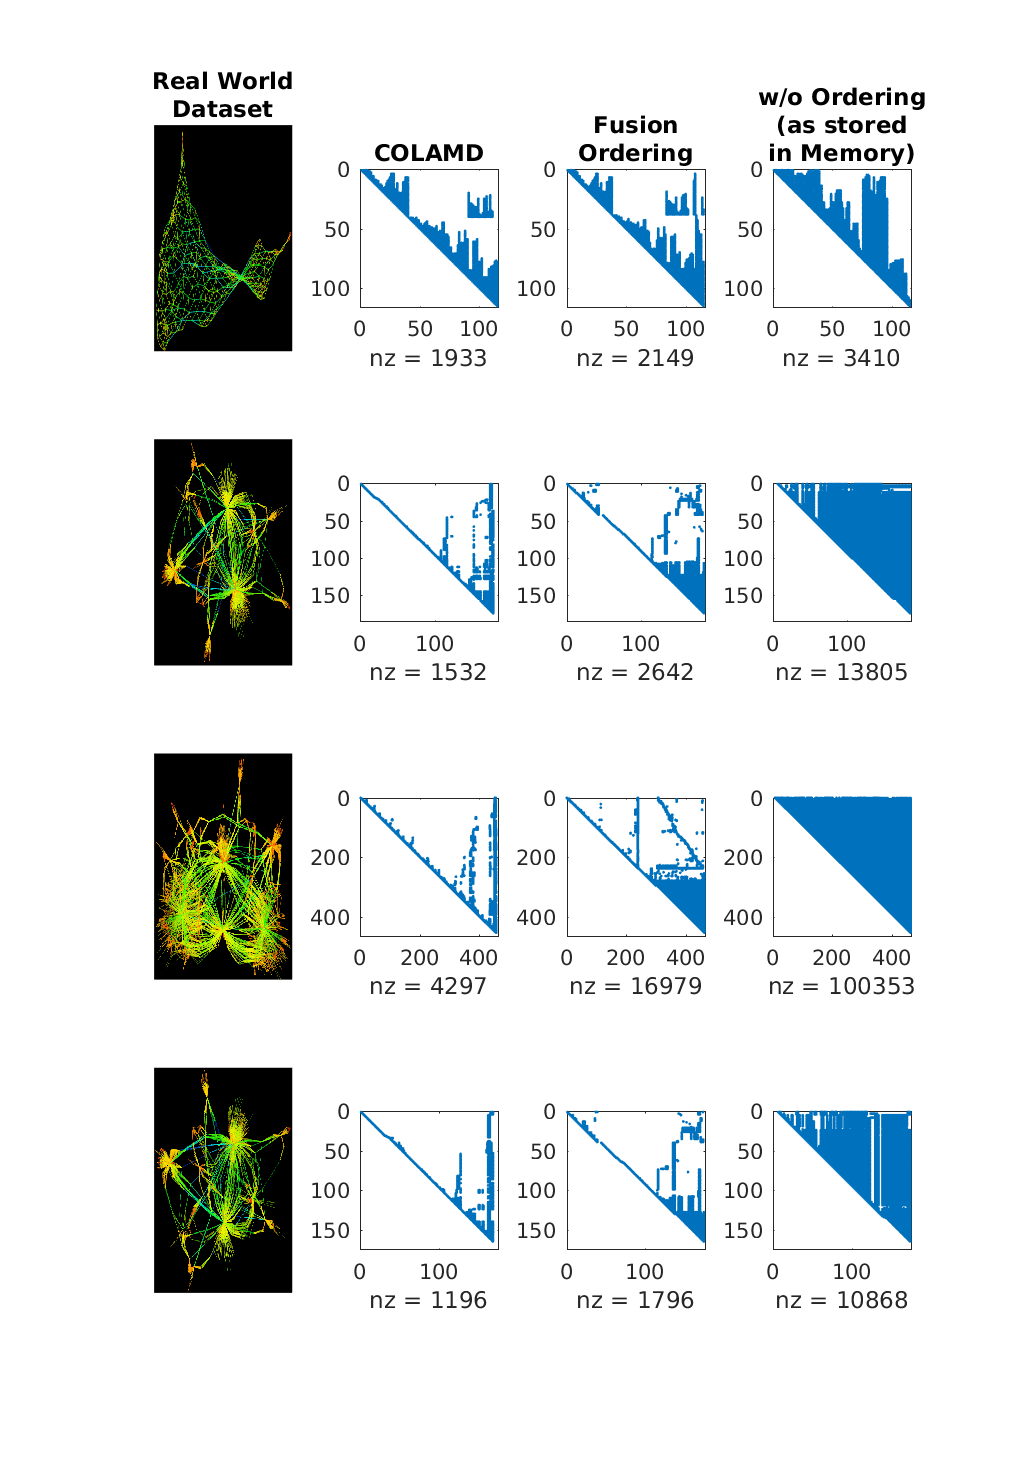
\includegraphics[width=\textwidth]{Chapters/figures3/ordering_comparison_1}
\caption{Comparison of number of non-zeros in the square root factor from QR factorization between the COLAMD ordering (second column), proposed ordering (third column) and the order in which the variables are retrieved (third column). The first column is the graph representation of the matrices in their lowest energy state \cite{suitesparse}.}
\label{fig:ordering_comparison_1}
\end{figure}
\begin{figure}[!]
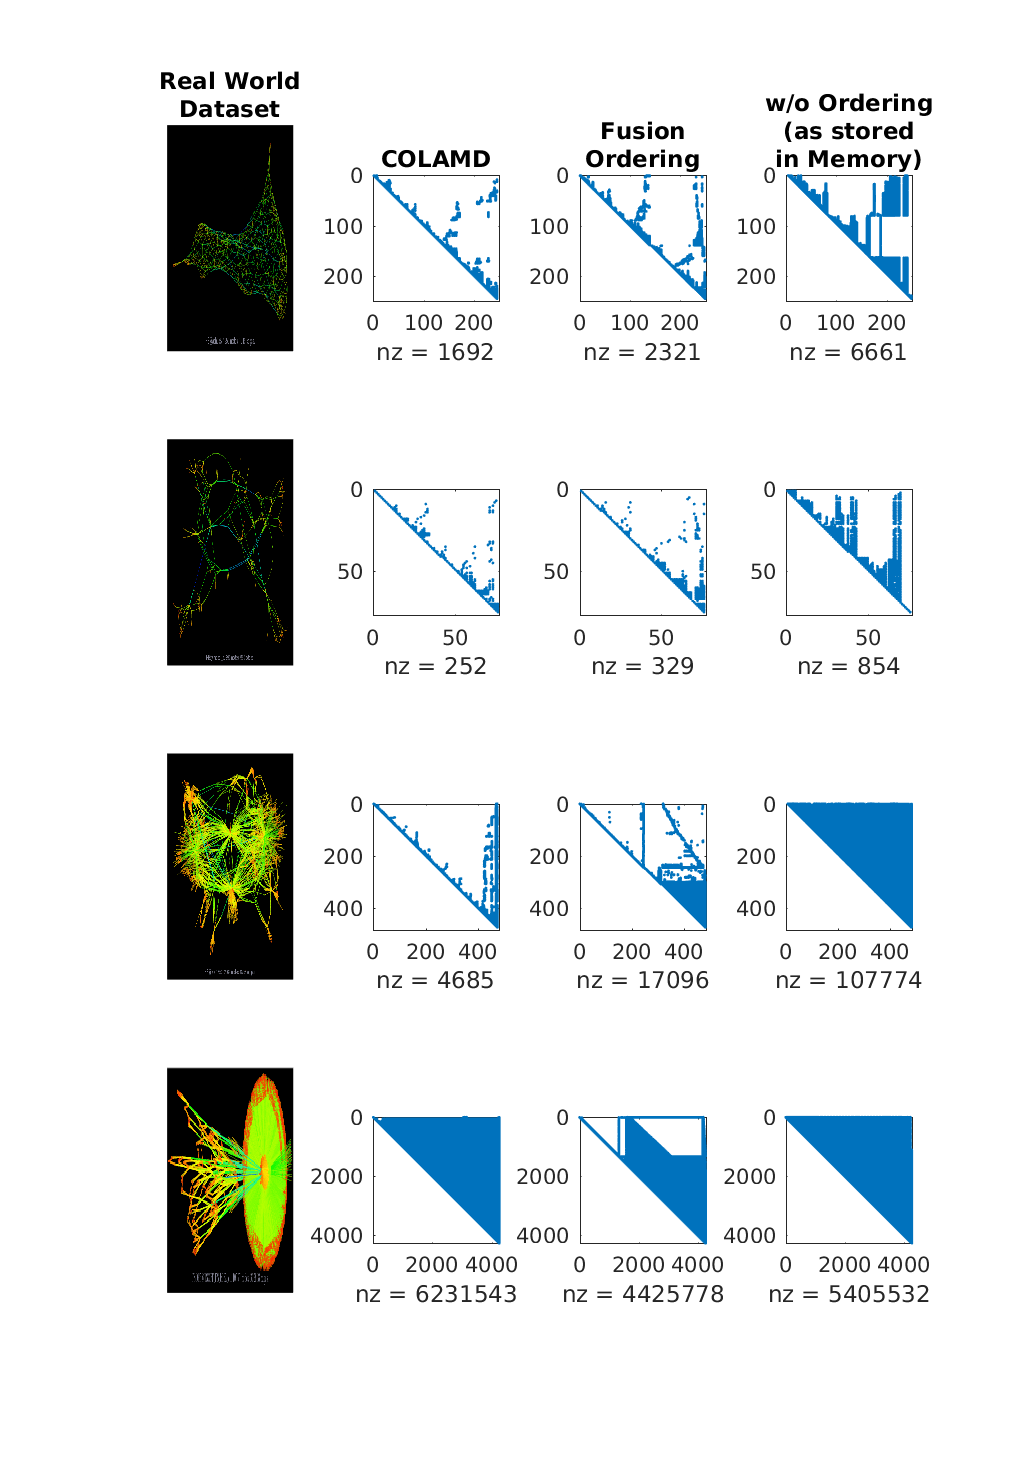
\includegraphics[width=\textwidth]{Chapters/figures3/ordering_comparison_2}
\caption{Comparison of number of non-zeros in the square root factor from QR factorization between the COLAMD ordering (second column), proposed ordering (third column) and the order in which the variables are retrieved (third column). The first column is the graph representation of the matrices in their lowest energy state \cite{suitesparse}.}
\label{fig:ordering_comparison_2}
\end{figure}
\paragraph{}
A comparison between the three types of orderings based on time taken to factorize the matrix after applying those ordering to the factor graph is performed in Figure \ref{fig:factorization_time}. As mentioned earlier, the orthonormal $Q$ matrix from QR decomposition is never explicitly formed in practice and hence the value of time is only that required to compute the square root factor $R$. Same experiment as before, comparing the number of non-zeros in the square root factor obtained from different ordering is also done on 120 real world matrices and plotted in Figure \ref{fig:nnz_comparison}. It can be seen that the proposed fusion ordering takes less time for factorization in many cases. This might be because the proposed ordering is inspired from variable ordering  by nested dissection and is compatible to parallel decomposition \cite{parallelqr}.
\begin{figure}[!]
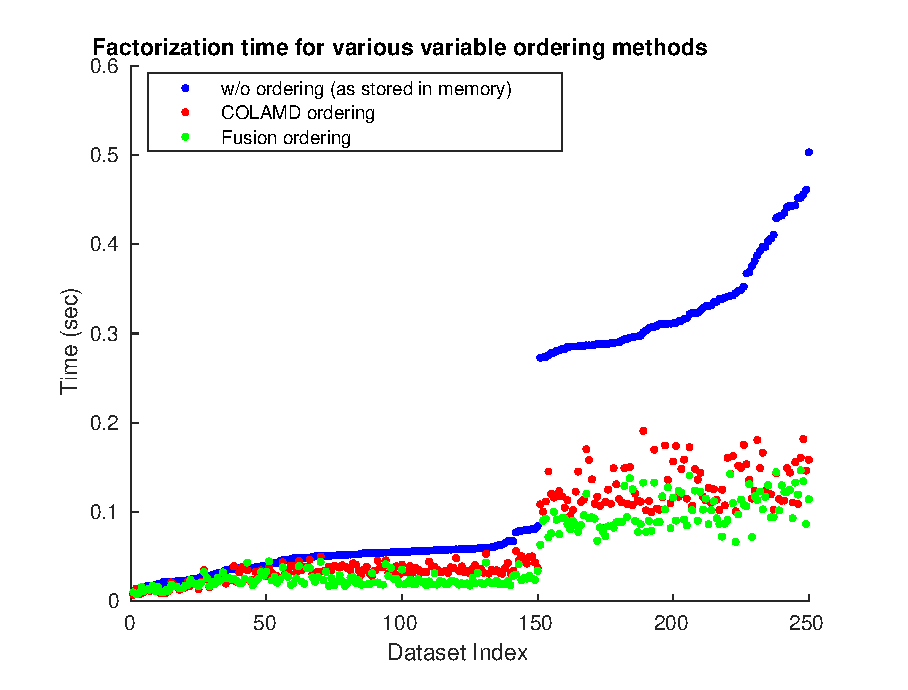
\includegraphics[width=\textwidth, height=0.4\textheight]{Chapters/figures3/factorization_time_comparison}
\caption{Comparison among different ordering schemes on the time taken to compute the square root factor $R$. It can be seen that the proposed fusion ordering takes less time than the COLAMD ordering as fusion ordering leaves the matrix in a state suitable for parallel QR decomposition \cite{parallelqr}.}
\label{fig:factorization_time}
\end{figure}
\begin{figure}[!]
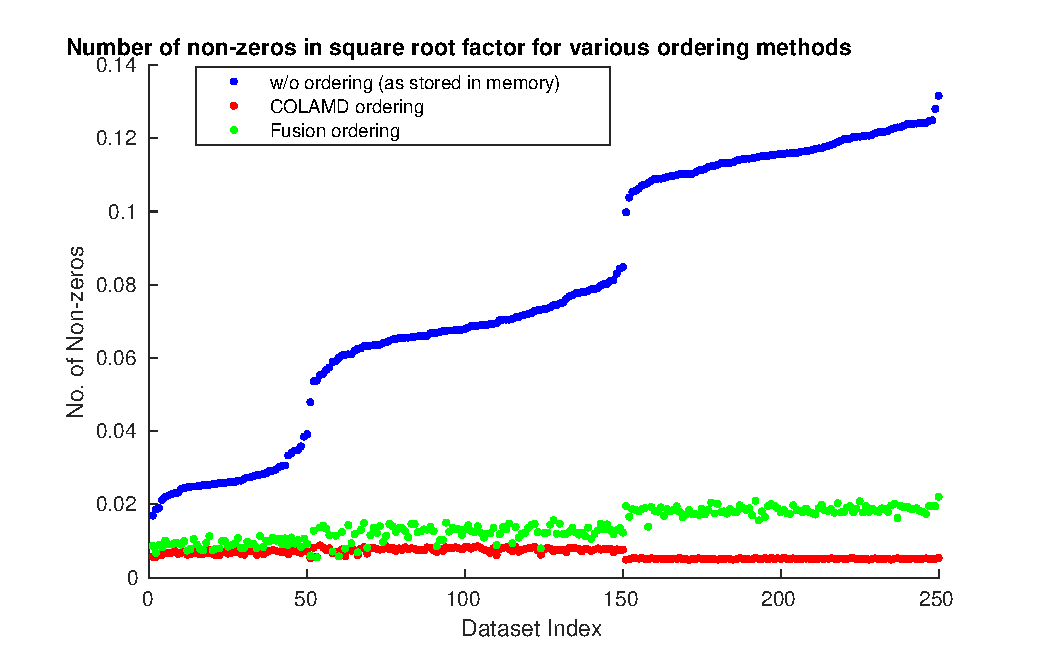
\includegraphics[width=\textwidth,  height=0.4\textheight]{Chapters/figures3/nnz_comparison}
\caption{Comparison among different ordering schemes on the number of non-zero fill-in produced. It can be seen that the COLAMD produces the least and is closely followed by fusion ordering. On the other hand, the variable memory order produces huge fill-in.}
\label{fig:nnz_comparison}
\end{figure}

%Relative ordering of c_affected 1 and c_affected 2 separately. c_2 affected is |c_1 affected| + argsort(c_2). Which sorted should be placed first out of two? The common elements placed at last.. Row ordering for stability... CFS like warranties?
%\newpage
%
%
%While combining the two graphs, \\
%Let $G^1 = (V^1, E^1)$ and $G^2 = (V^2, E^2)$ be the two graphs we are merging. Let $O^{G^1}$ and $O^{G^2}$ be their respective COLAMD orderings. Using these respective orderings the graphs $G^1$ and $G^2$ are stored as Bayes Tree. Let $C$ be the set of common nodes between the two graphs. Let $r_C^1$ and $r_C^2$ represent the set of nodes obtainedd from the Bayes Tree of $G^1$ and $G^2$ that gets affected on touching the common nodes $C$. The combined graph $G^C$ contains $V^C = C \cup r_C^1 \cup r_C^2$ and $E^C = E^p \cap (E^1 \cup E^2)$ where  $ E^p = \{ (v,w) \mid v \in V^C, w \in V^C, v \neq w\}$ is the power-set containing all the edges between nodes in $V^C$. \\
%
%\textbf{Relative Ordering:} As mentioned before, the ordering of the graph $G^1$ containing the vertices $V^1$ is given by $O^{G^1} = \{ o_1, o_2, ..., o_n \}$ where $n = \mid V^1\mid$. The relative ordering of the subgraph $S$ of the graph $G^1$ is given by 
%
%\begin{equation}
% O^S = arg sort(\bigcup_{v\in V^1} o^1(v))     
%\label{eq:relative}
%\end{equation}
%
%where $argsort$ gives the position of each element in the sorted array and $o^1(v)$ gives the order value of vertex $v \in V^1$ from the ordered set. $o^1(v)$ is equivalent to the value represented by $o$ with subscript $v$ in the set $O^1$. \\
%
%The combined graph ordering is done as follows - Let $O^{r_C^1}$, $O^{r_C^2}$ and $O^{C}$ be the relative ordering of $r_C^1$, $r_C^2$ and $C$ respectively. The relative ordering is calculated for $r_C^1$, $r_C^2$ and $C$ as shown in Eq. \ref{eq:relative} using their parent orderings $O^{G^1}$, $O^{G^2}$ and $O^{G^1}$ or $O^{G^2}$ respectively. This forms a block matrix as show in fig. \ref{fig:relative_colamd} that contains the nodes $r_C^1$, $r_C^2$ and $C$ in each of the blocks from left to right. The left top block contains the nodes in $r_C^1$ ordered using $O^{r_C^1}$, central bottom block contains $r_C^2$ ordered using $O^{r_C^2}$ and the right most block contains $C$ ordered using $O^C$. 
%
%\newpage
%
%Variable elimination [1, 4]
%originated in order to solve systems of linear equations, and was first applied in
%modern times by Gauss in the early 1800s [14]. [Related work]
%
%We also follow something like CCOLAMD to push the affected variable towards the end so as to reduce the computational steps in the upcoming updates. Tell this as though I did it. Put it as a part of HUND copy.
